\chapter{Tecnologías utilizadas}

\section{Visión general}

En esta sección se presentan las diferentes tecnologías que se han utilizado para el desarrollo del proyecto. Las principales tecnologías usado son las siguientes:

\section{Servidor MOAI}

MOAI\cite{MOAI} es una plataforma capaz de recolectar información de diversas fuentes y publicarlas mediante el protocolo \acrshort{oaipmh} desarrollado por Infrae\cite{Infrae} con el fin de satisfacer las necesidades de las instituciones académicas que trabajan con metadatos relacionales y ficheros de información.

\begin{figure}[!htbp]
	\centering
	
\includegraphics{fig/moai_logo}
	\caption{Logotipo de MOAI}
\end{figure}

Basado en un servidor \acrshort{http} Apache\cite{HTTPApache} e implementado en Python, MOAI incluye todas las funciones básicas como proveedor de datos del protocolo \acrshort{oaipmh}, indispensables para este proyecto. Por otra parte, permite tanto la extracción de la información de documentos \acrshort{xml} como recolectarla de diversos servidores de información tales como Fedora Commons\cite{Fedora}, EPrints\cite{EPrints} o DSpace\cite{DSpace} y almacenar la información cosechada en una base de datos SQLite\cite{SQLite} por defecto.

\subsection{Razón de uso}

Se ha escogido MOAI Server frete a las alternativas facilitadas por la misma comunidad de \acrshort{oai} en \url{https://www.openarchives.org/pmh/tools/tools.php} entre las que se cabe destacar a Fedora, EPrints y DSpace por las siguientes razones:

\begin{itemize}
	\item Su accesible documentación para el desarrollo y extensión del servidor.
	\item Capacidad para sobrescribir el esquema de la base de datos SQLite usado para la extracción de datos del servidor Apache por defecto y sustituirlo por la \acrshort{bd} PostgreSQL utilizada actualmente por LabMan, evitando replicar los datos.
	\item Implementado en una tecnología conocida, lo que reduce el tiempo de adaptación a la capa de datos.
\end{itemize}

\section{OAI-PMH validator}

\acrshort{oaipmh} validator\cite{oaipmh_validator} es una página web que permite validar el \acrshort{xml} generado por proveedores de datos de \acrshort{oaipmh} en desarrollo y comprobar si existe algún error en la estructura de la petición y si además realmente cumple con el estándar respetando el esquema \acrshort{oaipmh} y el formato bibliográfico \acrshort{dc}.


\begin{figure}[!htbp]
	\centering
	
\includegraphics[scale=0.5]{fig/oaipmh_validator_logo}
	\caption{Logotipo de \acrshort{oaipmh} validator}
\end{figure}

La aplicación web permite validar como descargar la petición resultante a partir de las \acrshortpl{url} de servidores públicos de forma gratuita, permitiendo realizar cinco de las seis operaciones que establece el protocolo \acrshort{oaipmh}. Además facilita la validación directa de fuentes \acrshort{xml} generados por servidores que aún están en pruebas y no son públicos también de forma gratuita. A modo de aclaración, en la figura \ref{fig:oai_validator} se muestra un ejemplo de una validación del comando \textit{ListMetadataFormats} mediante una consulta POST a el repositorio \url{https://dspace.lib.uom.gr/dspace-oai/request}.

\begin{figure}[!htbp]
	\centering
	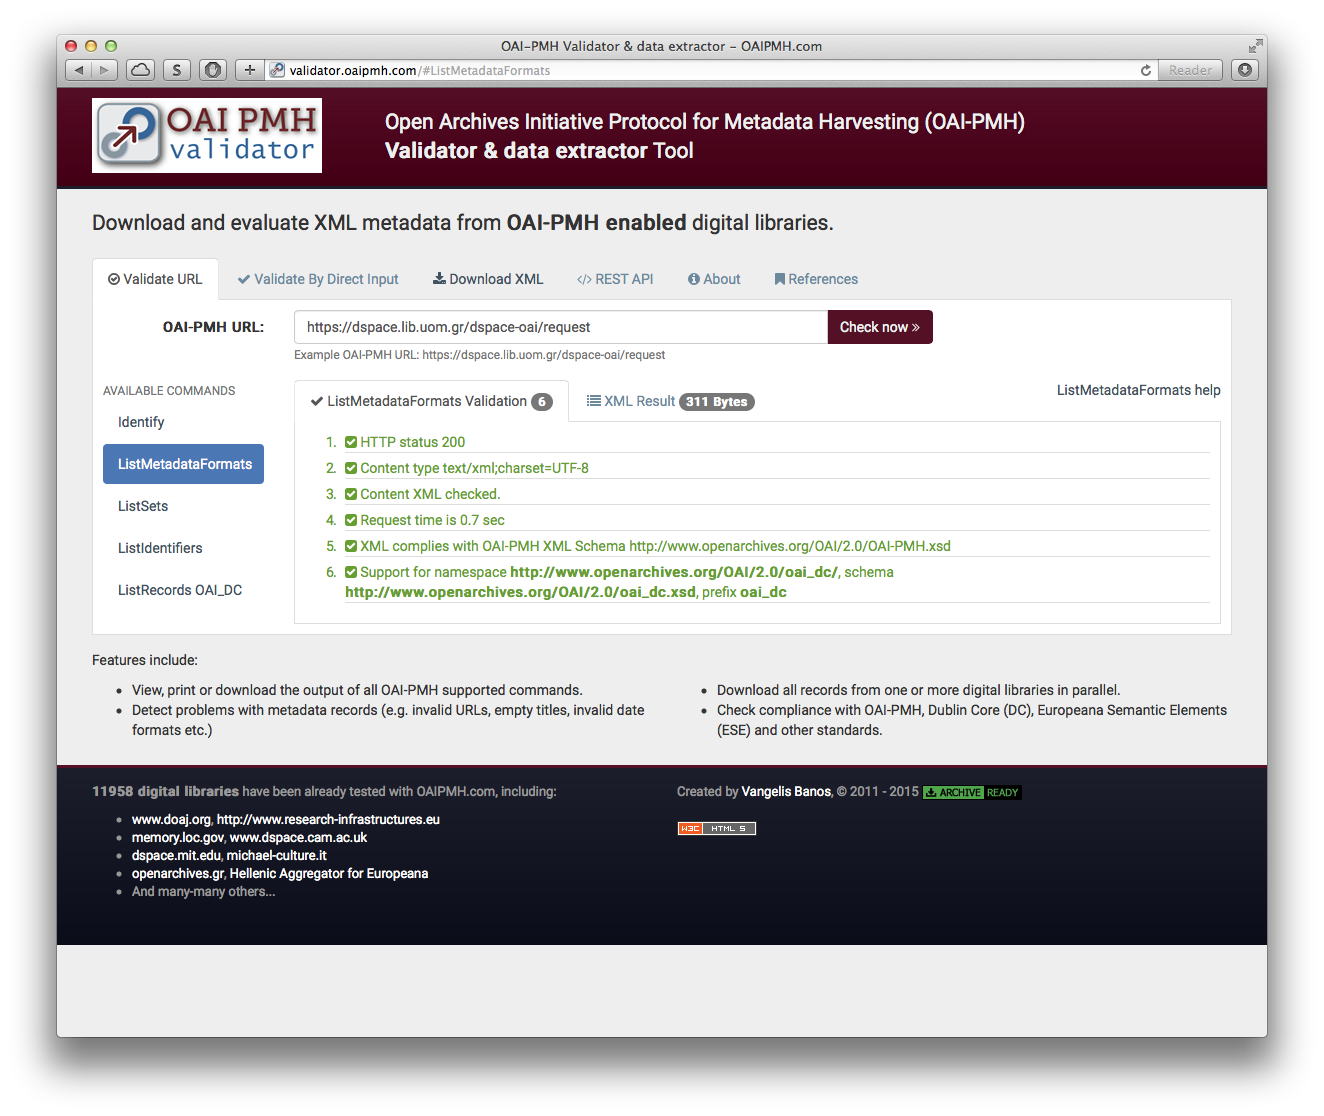
\includegraphics[scale=0.25]{fig/oaipmh_validator_example}
	\caption{Ejemplo de validación de una consulta en \acrshort{oaipmh} validator}
	\label{fig:oai_validator}
\end{figure}

\subsection{Razón de uso}

Se ha utilizado esta aplicación web frente a los distintos validadores existentes como Oval\cite{Oval}, principalmente por que ha permitido comprobar la velidez de los \acrshortpl{xml} generados por el proveedor de información, en la etapa de desarrollo en el que el servidor no era público y por tanto no disponía de una \acrshort{url} a la que hacer referencia para realizar dichas comprobaciones.

\section{SQLAlchemy}

SQLAlchemy\cite{SQLAlchemy} consiste tanto en \acrfull{orm} como en un juego de herramientas \acrshort{sql} para el lenguaje de programación Python. Como los propios desarrolladores definen ``SQLAlchemy ofrece una \textit{suite} completa de patrones de persistencia, diseñada para una acceso eficiente y de alto rendimiento a la \acrlong{bd}, adaptado a lenguaje sencillo como lo es Python''

\begin{figure}[!htbp]
	\centering
	
\includegraphics[scale=0.5]{fig/sqla_logo}
	\caption{Logotipo de SQLAlchemy}
\end{figure}

\subsection{Razón de uso}

Se ha utilizado esta \acrshort{api} frente a otras soluciones, como puede ser el \acrshort{orm} de Django, principalmente por las siguientes razones:

\begin{itemize}
	\item Ofrece un nivel de abstracción mayor manipulando las tablas de la \acrshort{bd} como si de objetos de Python se tratasen.
	\item Permite escoger el grado de abstracción deseado, pudiendo escoger entre las herramientas \textit{core}, para la manipulación de tablas, o del \acrshort{orm} para gestionar el propio modelo de la \acrshort{bd} como objetos.
	\item Es uno de los \acrshortpl{orm} más usados, utilizado por organizaciones como Mozilla\cite{Mozilla} o Reddit\cite{Reddit}.
	\item Ofrece una documentación detallada tanto para el uso de las herramientas \textit{core} como para aquellas relacionadas con el \acrshort{orm} en sí. Además debido a ser una de las herramientas más usadas dispone de una gran comunidad que está dispuesta a ayudar a resolver cualquier problema.
	\item Soporta desde Python 2.5 hasta las últimas versiones 3.x del mismo.
	\item SQLAlchemy incluye dialectos para \acrlongpl{bd} como SQLite, PostgreSQL, MySQL, Oracle\cite{Oracle}, MS-SQL\cite{MSSQL}, Firebird\cite{Firebird} y muchas otras por medio de extensiones, por lo que las clases generadas con esta herramienta pueden ser reutilizadas en caso de migración a una de estas \acrshort{bd}.
	\item Estaba integrado como una dependencia por el servidor de MOAI lo que evitaba los quebraderos de cabeza de tener que instalar otros \acrshortpl{orm}
\end{itemize}

\section{Django}

Django es un \textit{framework open-source} para el desarrollo de aplicaciones web escrito en Python y basado en el patrón \acrfull{mvc}. El principal objetivo de Django, es facilitar el proceso de creación de paginas web complejas enfatizando especialmente en la reusabilidad y en la modularidad de sus componentes bajo el lema inglés \acrfull{dry}.

\begin{figure}[!htbp]
	\centering
	
\includegraphics[scale=0.18]{fig/django_logo}
	\caption{Logotipo de Django}
\end{figure}

\subsection{Razón de uso}

Se ha utilizado este entorno de desarrollo frente a otras soluciones, como puede ser \acrfull{ror}\cite{RoR} o más modernas como Express\cite{Express} por las siguientes razones:

\begin{itemize}
	\item Es usado por grandes páginas como Mozilla, The Washington Times\cite{TWT} o Bitbucket\cite{Bitbucket}.
	\item El \acrshort{orm} de Django es una herramienta para la gestión de las \acrlongpl{bd} extremadamente potente, además de ser es una de las más usadas en la comunidad de Python.
	\item La interfaz de administración es muy potente y personalizable por lo que ahorra mucho tiempo de desarrollo.
	\item Principalmente por que \acrshort{labman} está desarrollado en esta tecnología y para extenderla se ha tenido que trabajar con ella para no desechar lo que ya estaba hecho.
\end{itemize}

\section{jQuery}

jQuery\cite{jQuery} es una librería multiplataforma gratuita de \acrfull{js} diseñada para simplificar el desarrollo de la parte cliente. La sintaxis de jQuery está pensada para facilitar la navegación por el árbol de elementos del \acrfull{dom}, proporcionando funciones para la manipulación de los mismos. El objetivo de jQuery es poder realizar todas las operaciones que se podría realizar con \acrshort{js} teniendo que escribir mucho menos código para conseguirlo.

\begin{figure}[!htbp]
	\centering
	\includegraphics[scale=0.6]{fig/jquery_logo}
	\caption{Logotipo de JQuery}
\end{figure}

\subsection{Razón de uso}

Se ha utilizado esta \acrshort{api} de \acrshort{js} frente a otras posibles soluciones, como puede Prototype\cite{Prototype} por las siguientes razones:

\begin{itemize}
	\item jQuery es una tecnología intuitiva, fácil de aprender que simplifica el código además del tiempo de desarrollo de la aplicación.
	\item Tiene una gran comunidad por detrás que crea infinitos tutoriales para ayudar a los desarrolladores novatos a dar sus primeros pasos.
	\item jQuery es una librería multiplataforma y compatible con todos los navegadores web que se encarga de solucionar los problemas de \acrshort{js} presentes en las primeras versiones de Firefox\cite{Firefox} o \acrfull{ie}\cite{IE}, permitiendo escribir el código una sola vez para todos los navegadores.
\end{itemize}

\section{Bootstrap}

Bootstrap en un \textit{framework} gratuito para la creación de aplicaciones web que contiene unas plantillas, basadas en \acrshort{html} y \acrshort{css}, para formularios, botones, navegación y muchos otros tipos de componentes de la interfaz gráfica, así como extensiones \acrshort{js}. El objetivo de Bootstrap es facilitar el desarrollo web ofreciendo la posibilidad de generar interfaces de usuario con aspecto visual atractivo sin la necesidad de disponer de nociones de diseño gráfico.

\begin{figure}[!htbp]
	\centering
	
\includegraphics[scale=0.45]{fig/bootstrap_logo}
	\caption{Logotipo de Bootstrap}
\end{figure}

Fue creado por dos desarrolladores en Twitter para fomentar la consistencia entre las herramientas internas y fue publicado como código abierto más adelante, convirtiéndose en uno de los \textit{framework} de desarrollo web más destacados.

Además, para complementar a Bootstrap se han utilizado las siguientes extensiones para resolver ciertos problemas en la consistencia del \textit{look and feel} de varios componentes y añadir nuevas funciones:

\subsection{Bootstrap-select}

Bootstrap-select\cite{BootstrapSelect} es una extensión que añade el estilo característico de Bootstrap las etiquetas \textit{select} de \acrshort{html}, sobrescribiendo el estilo dependiente del sistema operativo que disponen por defecto. 

Este \textit{plugin} no solo altera el aspecto visual del componente de selección, sino que, por otra parte añade la posibilidad disponer los elementos en agrupaciones, añadir validaciones como un máximo y mínimo de elementos seleccionados y facilitar la modificación del componente mediante \acrshort{js}.

\begin{figure}[!htbp]
	\centering
	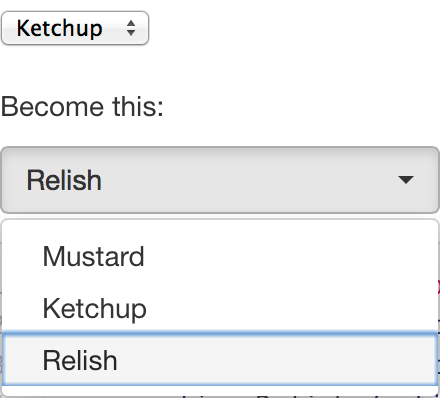
\includegraphics[scale=0.45]{fig/bootstrap_select}
	\caption{Cambio visual producido por Bootstrap-select}
	\label{fig:bootstrap-select}
\end{figure}

\FloatBarrier

En la figura \ref{fig:bootstrap-select} puede observarse el cambio visual que sufre el componente \text{select} renderizado bajo Safari\cite{Safari}.

\subsection{Bootstrap 3 Datepicker}

Bootstrap 3 Datepicker\cite{BootstrapDatepicker} es una extensión que combina varios elementos de Bootstrap y le añade la funcionabilidad de un \textit{input date} nativo de \acrshort{html}5 manteniendo así la armonía estética característica de Bootstrap.

\begin{figure}[!htbp]
	\centering
	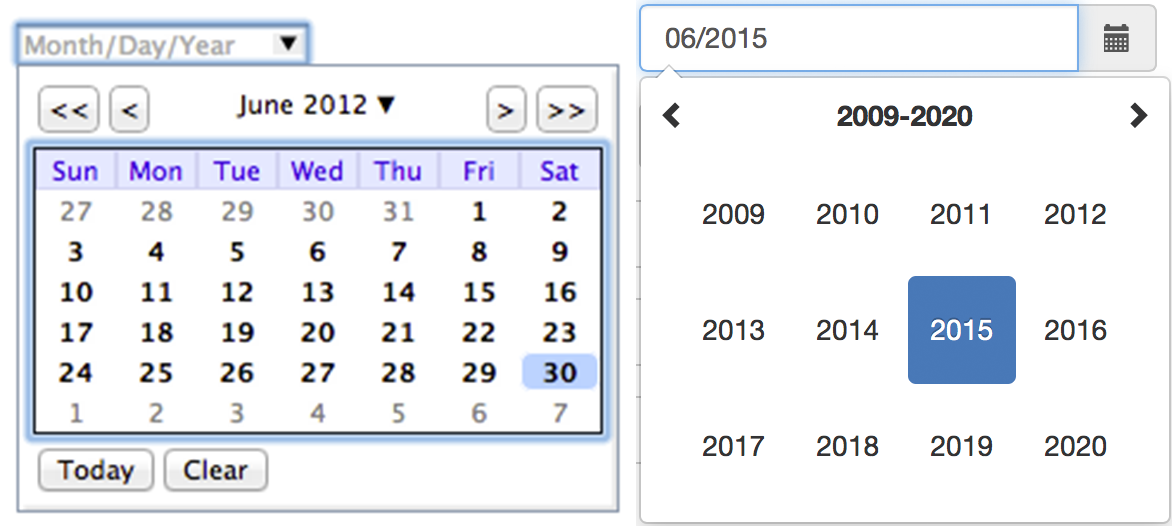
\includegraphics[scale=0.25]{fig/bootstrap_datepicker}
	\caption{Cambio visual producido Bootstrap 3 Datepicker}
	\label{fig:bootstrap-datepicker}
\end{figure}

Además de otorgar un cambio visual, tal y como puede observarse en la figura \ref{fig:bootstrap-datepicker}, esta \acrshort{api} aporta facilidades para la manipulación de los atributos de este componente, así como la gestión de eventos.

\subsection{Razón de uso}

Se ha utilizado este \textit{framework} para el diseño del \textit{front-end} frente a otras posibles soluciones, como puede Skeleton\cite{Skeleton} por las siguientes razones:

\begin{itemize}
	\item Aumenta la velocidad del desarrollo. Al facilitar el diseño de muchos de los componentes \acrshort{html} para formularios, tipográficas, etc. el desarrollador puede desentenderse de apartado artístico y dedicarse a la lógica de la aplicación web.
	\item A partir de la versión 2.0 de Bootstrap ofrece soporte responsivo, es decir, la capacidad para adaptarse a múltiples dispositivos, como pueden ser tabletas, equipos de sobremesa, dispositivos móviles, teniendo que desarrollar una única vez el apartado gráfico.
	\item El soporte, Bootstrap ha acumulado tras de sí una gran comunidad que está dispuesta a solucionar cualquier problema que pueda surgir durante el desarrollo de interfaces gráficas.
	\item Comunidad de desarrolladores artísticos, Bootstrap dispone miles de artistas que diseñan plantillas para páginas web gratuitas pudiendo ser modificadas a las necesidades del producto en desarrollo.
	\item Dispone de un sistema de rejillas para la disposición de elementos, que facilita la disposición de los elementos en pantalla y que a su vez se adapta a las pantallas de los dispositivos, pudiendo evitar los quebraderos de cabeza que supone modificar \acrshort{css} y añadir \textit{media queries} para obtener el mismo resultado.
	\item Se ha usado está tecnología dado que \acrshort{labman} estaba desarrollado en esta y era requisito indispensable mantener el \textit{look and feel} de la aplicación en armonía.
\end{itemize}
